\documentclass[a4paper,11pt]{article}
\usepackage{amsmath}
\usepackage{amssymb}
\usepackage{placeins}
\usepackage{array}
\usepackage{hyperref}
\usepackage{graphicx}
\usepackage{units}
\usepackage{xfrac}
\usepackage[version=4]{mhchem}
\usepackage[margin=0.9in]{geometry,caption}
\usepackage{braket}
\usepackage{gensymb}
\usepackage{wasysym}
\usepackage{tikz}
\usepackage{physics}
\usepackage{booktabs}
\usepackage{multirow}
\usepackage{subcaption}
\usepackage[capitalise,
					 noabbrev]{cleveref}
\usepackage[mathlines]{lineno}
\usepackage{cleveref}
 \usepackage{setspace}
 \usepackage{bm}
\usepackage{fancyhdr}
\usepackage{makecell}
\usepackage{setspace}
\usepackage{chngcntr}
\usepackage{afterpage}
\usepackage{CJKutf8}
\usepackage{bm}
\usepackage{tocloft}
\setlength{\cfttabnumwidth}{1.5cm}
\setlength{\cftfignumwidth}{1.5cm}

\renewcommand*\thetable{\Roman{table}}


%%%Add this for version history
%\setcounter{section}{-1}

%%spacing on tilde for approximate values
\let\oldsim\sim 
\renewcommand{\sim}{{\oldsim}}

%%1.5 spacing
\onehalfspacing

\pagestyle{fancy}
\fancyhf{}
\setlength{\headheight}{14pt}
\fancyhead[L]{\nouppercase\leftmark}
\fancyhead[L]{\nouppercase\rightmark}
%\fancyhead[ER,OL]{\nouppercase\rightmark}
\rhead{\thepage}


%%%Patch AMSmath environments to work correctly with lineno
\usepackage{etoolbox}
\newcommand*\linenomathpatchAMS[1]{%
  \expandafter\pretocmd\csname #1\endcsname {\linenomathAMS}{}{}%
  \expandafter\pretocmd\csname #1*\endcsname{\linenomathAMS}{}{}%
  \expandafter\apptocmd\csname end#1\endcsname {\endlinenomath}{}{}%
  \expandafter\apptocmd\csname end#1*\endcsname{\endlinenomath}{}{}%
}

\expandafter\ifx\linenomath\linenomathWithnumbers
  \let\linenomathAMS\linenomathWithnumbers
  %% The following line gets rid of an extra line numbers at the bottom:
  \patchcmd\linenomathAMS{\advance\postdisplaypenalty\linenopenalty}{}{}{}
\else
  \let\linenomathAMS\linenomathNonumbers
\fi
\linenomathpatchAMS{align}

\graphicspath{{images/}}

\begin{document}

\title{\huge{HK-TN-???: HK LI Fibre Specifications}}
\author{S. J. Jenkins, B. Bogdan, N. Foster, N. K. McCauley}

\maketitle

\tableofcontents

\newpage

\section{Introduction}\label{sec:intro}
The Hyper-Kamiokande experiment has a broad physics program, including the aim of making precision measurements of neutrino oscillation parameters. In order to make such precision measurements, a precise understanding of the detector itself is required. To this end an array of different calibration systems are planned, with each playing a crucial role in driving systematic uncertainties down to the percent-level required.

A key component of the calibration program is the light injection (LI) system, which has two primary aims. The first is to measure the optical properties of the water in the tank, and monitor how the measured absorption and scattering parameters evolve with time. The second is to provide light sources with which to calibrate PMT response. In order to illuminate the injectors, lengths of fibre optic cable will be used to carry light from the sources on the top of the tank, all the way to the injectors installed on the PMT support structure.

This technical note focuses on the fibre optic requirements for the LI system, describing the quantities and lengths of cables needed, along with the lab measurements performed to decide on which types of fibre optic cables to use.

\section{HK LI System Overview}\label{sec:overview}

The HK LI system will be split into two parts, one for the inner detector (ID) and one for the outer detector (OD). The ID system will consist of 33 injector positions, each housing a diffuser and collimator. Full details of the diffuser and collimator designs and requirements can be found in HK-TN-0042 \cite{bib:tn0042} and HK-TN-0065 \cite{bib:tn0065}, respectively. 28 injector positions will be located in the barrel region, with 7 locations equally spaced in $z$, each having four positions equally spaced in $\theta$. The bottom end-cap will feature four more injector locations, with the injectors all facing upwards in the $+z$ direction. The top end-cap will feature a single location, where a calibration port will be used, rather than fixing to the PMT support structure. \cref{fig:IDmap} shows the injector locations described.
\begin{figure}[h]
\centering
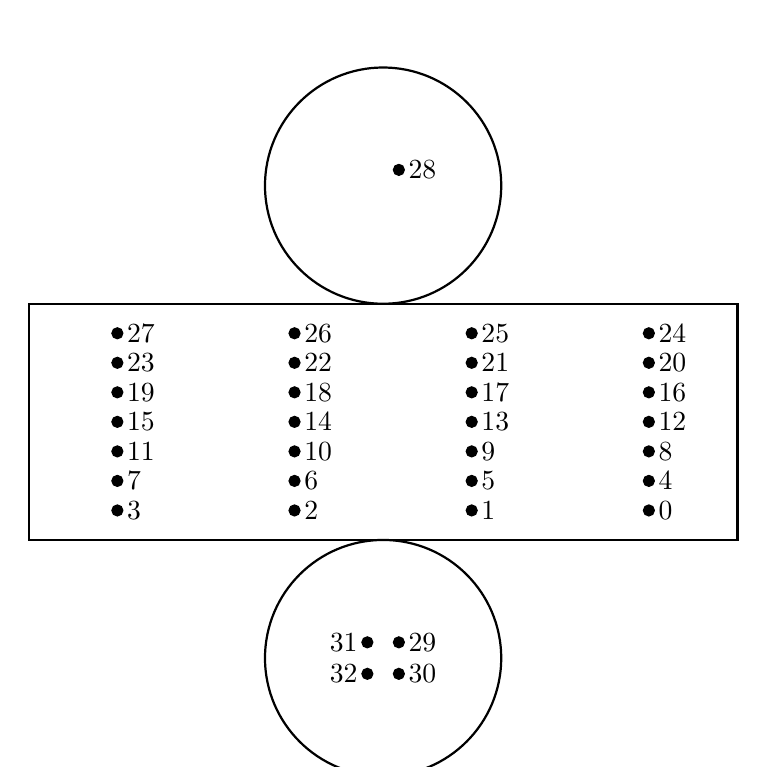
\begin{tikzpicture}
\draw[thick] (-4.5, -1.5) rectangle (4.5, 1.5);
\draw[thick] (0, 3) circle (1.5cm);
\draw[thick] (0, -3) circle (1.5cm);
\filldraw[black] (3.375, -1.125) circle (2pt) node[anchor=west]{0};
\filldraw[black] (3.375, -0.75) circle (2pt) node[anchor=west]{4};
\filldraw[black] (3.375, -0.375) circle (2pt) node[anchor=west]{8};
\filldraw[black] (3.375, 0) circle (2pt) node[anchor=west]{12};
\filldraw[black] (3.375, 0.375) circle (2pt) node[anchor=west]{16};
\filldraw[black] (3.375, 0.75) circle (2pt) node[anchor=west]{20};
\filldraw[black] (3.375, 1.125) circle (2pt) node[anchor=west]{24};
\filldraw[black] (1.125, -1.125) circle (2pt) node[anchor=west]{1};
\filldraw[black] (1.125, -0.75) circle (2pt) node[anchor=west]{5};
\filldraw[black] (1.125, -0.375) circle (2pt) node[anchor=west]{9};
\filldraw[black] (1.125, 0) circle (2pt) node[anchor=west]{13};
\filldraw[black] (1.125, 0.375) circle (2pt) node[anchor=west]{17};
\filldraw[black] (1.125, 0.75) circle (2pt) node[anchor=west]{21};
\filldraw[black] (1.125, 1.125) circle (2pt) node[anchor=west]{25};
\filldraw[black] (-3.375, -1.125) circle (2pt) node[anchor=west]{3};
\filldraw[black] (-3.375, -0.75) circle (2pt) node[anchor=west]{7};
\filldraw[black] (-3.375, -0.375) circle (2pt) node[anchor=west]{11};
\filldraw[black] (-3.375, 0) circle (2pt) node[anchor=west]{15};
\filldraw[black] (-3.375, 0.375) circle (2pt) node[anchor=west]{19};
\filldraw[black] (-3.375, 0.75) circle (2pt) node[anchor=west]{23};
\filldraw[black] (-3.375, 1.125) circle (2pt) node[anchor=west]{27};
\filldraw[black] (-1.125, -1.125) circle (2pt) node[anchor=west]{2};
\filldraw[black] (-1.125, -0.75) circle (2pt) node[anchor=west]{6};
\filldraw[black] (-1.125, -0.375) circle (2pt) node[anchor=west]{10};
\filldraw[black] (-1.125, 0) circle (2pt) node[anchor=west]{14};
\filldraw[black] (-1.125, 0.375) circle (2pt) node[anchor=west]{18};
\filldraw[black] (-1.125, 0.75) circle (2pt) node[anchor=west]{22};
\filldraw[black] (-1.125, 1.125) circle (2pt) node[anchor=west]{26};
\filldraw[black] (0.2, 3.2) circle (2pt) node[anchor=west]{28};
\filldraw[black] (0.2, -2.8) circle (2pt) node[anchor=west]{29};
\filldraw[black] (0.2, -3.2) circle (2pt) node[anchor=west]{30};
\filldraw[black] (-0.2, -2.8) circle (2pt) node[anchor=east]{31};
\filldraw[black] (-0.2, -3.2) circle (2pt) node[anchor=east]{32};
\end{tikzpicture}
\caption{Injector location map for ID positions. Each location will feature a diffuser and collimator.}\label{fig:IDmap}
\end{figure}
Installing injectors at different heights throughout the detector will allow water parameters to be measured as a function of depth.

The OD system will consist primarily of diffusers, using bare hemispheres coupled to fibres, rather than the housed versions used for the ID system. 122 of these OD diffusers will be installed, with the current design featuring 84 equally spaced around the barrel region. This results in 7 rows of 12 diffusers, with rows alternately offset from one another. This configuration is particularly advantageous as it matches the number of rows in the ID system, simplifying the installation of the fibre optic cables. Each end-cap would then feature 19 diffusers, again equally spaced across the surface. A diagram showing this layout is presented in \cref{fig:ODdiffmap}. Finally, 12 collimators will be installed in the OD, in suitable locations to achieve long path lengths such as across the end caps and up the side of the barrel. These collimators will be exactly the same as those installed in the ID.

\begin{figure}[h]
\centering
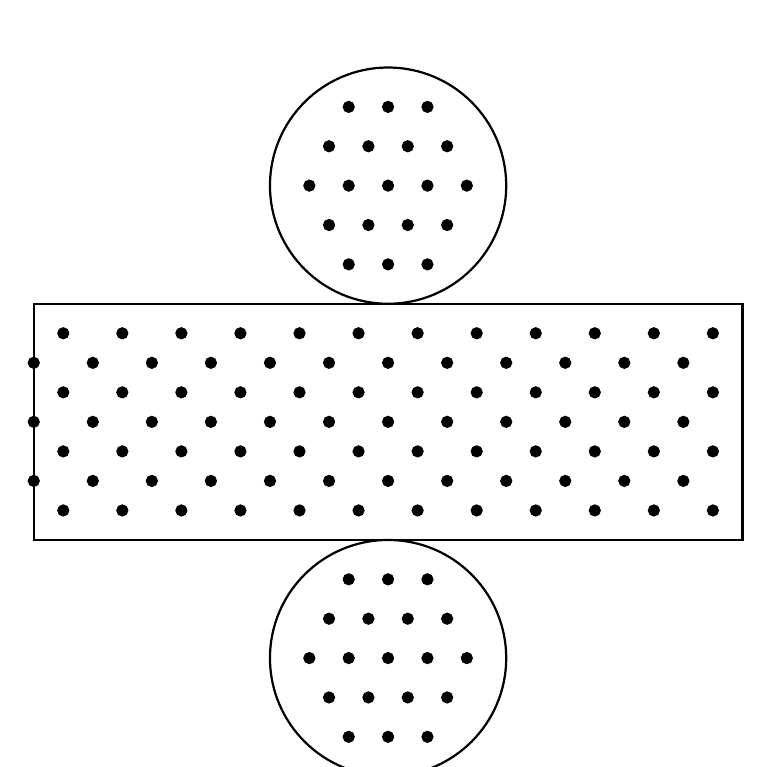
\begin{tikzpicture}
\draw[thick] (-4.5, -1.5) rectangle (4.5, 1.5);
\draw[thick] (0, 3) circle (1.5cm);
\draw[thick] (0, -3) circle (1.5cm);
%barrel locations
\foreach \x in {0,...,11}{
	\foreach \y in {0,...,6}{
		\ifodd \y \filldraw[black] (-4.5+\x*2*0.375, -1.125+\y*0.375) circle (2pt);
		\else \filldraw[black] (-4.5+0.375+\x*2*0.375, -1.125+\y*0.375) circle (2pt);
		\fi
		}
	}
%topcap
\foreach \y in {0,...,2}{
	\foreach \x in {0,...,2}{
		\filldraw[black] (-0.5+\x*0.5, 1.5+0.5+2*\y*0.5) circle (2pt);
		}
	}
\foreach \y in {0,...,1}{
	\foreach \x in {0,...,3}{
		\filldraw[black] (-0.75+\x*0.5, 1.5+2*0.5+2*\y*0.5) circle (2pt);
		}
	}
\foreach \x in {0,...,1}{
	\filldraw[black] (-1+\x*2, 3) circle (2pt);
	}
%bottom cap
\foreach \y in {0,...,2}{
	\foreach \x in {0,...,2}{
		\filldraw[black] (-0.5+\x*0.5, -1.5-0.5-2*\y*0.5) circle (2pt);
		}
	}
\foreach \y in {0,...,1}{
	\foreach \x in {0,...,3}{
		\filldraw[black] (-0.75+\x*0.5, -1.5-2*0.5-2*\y*0.5) circle (2pt);
		}
	}
\foreach \x in {0,...,1}{
	\filldraw[black] (-1+\x*2, -3) circle (2pt);
	}
\end{tikzpicture}
\caption{Injector location map for OD diffuser positions. Locations are approximate and dependent on PMT/WLS plate locations.}\label{fig:ODdiffmap}
\end{figure}

In order to illuminate the injectors, two separate systems will be employed. The first of these will be a system formed of six picosecond pulsed laser sources, in the wavelength range 337 -- 550 nm. This laser system will be used to illuminate all of the ID injectors, along with the 12 OD collimators. {\color{red} put further details on switches and setup in a different section?}. The OD diffusers on the other hand will be illuminated by an LED pulser system, utilising a series of 365~nm wavelength LEDs. Both of these systems will feature monitoring devices, so that the stability of the light sources can be monitored prior to convolution with detector parameters.


\section{Fibre Lab Measurements}

In order to make an informed decision on the optimal fibres to use for the LI system in HK, a series of measurements were made of the properties of the candidate fibres chosen. This section describes the fibre test stand setup at University of Liverpool, along with the measurements made of the candidate fibres, before discussing the decision on which fibres to use.

For the fibres to be suitable for use in the LI system, there are a series of requirements. These are:
\begin{itemize}
\item The fibre should be capable of transporting light of wavelengths in the range 337 -- 550~nm.
\item The attenuation of the input signal across the full length of fibre should be minimised
\item The dispersion of the input signal across the full length of fibre should be minimised {\color{red} these really need quantifying, somehow}
\end{itemize}

Six different fibre types from Thorlabs were considered. Four of these were step-index fibres; two wide-core fibres (FP200URT and FP400URT) and two narrow-core fibres (FG050UGA and FG105UCA) were chosen. The remaining two candidates were graded-index fibres (GIF50C and GIF50D). The reason for the inclusion of these was to confirm whether a graded-index fibre core is required in order to limit dispersion. The main specifications of each fibre type are summarised in \cref{tab:fibres}. GIF50C and GIF50D have almost the same specifications, with the only difference being the available bandwidth.
\begin{table}[h]
\centering
\begin{tabular}{llccc}
\hline
Fibre	   & Type   		  & Core \diameter [$\mu$m] &  NA 	  &  Transmission region [nm]\\ \hline
FG050UGA   &  Step-index      &           \phantom{0}50  			&  0.22   &   250--1200       \\
FG105UCA   &  Step-index      &           105  			&  0.22   &   250--1200       \\
FP200URT   &  Step-index      &           200  			&  0.50   &   300--1200       \\
FP400URT   &  Step-index      &           400  			&  0.50   &   300--1200      \\
GIF50C     &  Graded-index    &           \phantom{0}50  			&  0.20	  &   800--1600       \\
GIF50D     &  Graded-index    &           \phantom{0}50 			&  0.20   &   800--1600      \\ \hline
\end{tabular}
\caption{Fibre types used for initial testing in lengths of 1~m and 35~m.}\label{tab:fibres}
\end{table}
Preliminary measurements were performed with all six fibre types listed, and these results were used to make an informed choice on which should be investigated more thoroughly.


\subsection{Fibre Test Stand}\label{sec:meas:sub:stand}

All fibre measurements were performed using the fibre test stand in the Particle Physics Optical Laboratory at the University of Liverpool. Two different types of light sources are available for testing; the first of these is a Picoquant Sepia PDL 828-L laser driver, powering a LDH-D-C-375M laser head, with a peak wavelength of 371~nm. This is a pulsed laser source with a pulse width of $\sim$50~ps, and repetition rate up to 80~MHz. The candidate fibres couple directly to the laser head using an FC/PC connector. The second set of light sources was a series of LEDs, covering wavelengths from 365~nm up to 595~nm. These are run in DC mode, and were used primarily to make attenuation measurements over the range of wavelengths relevant for the LI system. In order to connect the FC/PC connector on a candidate fibre to a surface-mounted LED, custom connectors were 3D printed. {\color{red} does this need expanding?}

Two different detection methods for the fibre transmitted light are available. To measure power output, a Thorlabs PM100USB power meter is used, with an S150C sensor connected. For timing measurements, the fibres are connected to a Hamamatsu H10721-110 PMT, which is read out by a Tektronix MSO56{\color{red} check model no.} oscilloscope. Fibres are coupled to either read-out method via FC/PC connection such that, in the case of the laser, there are no bare beams in the lab. To ensure light tightness and as an additional safety measure, all light sources and detectors are housed within a dark box, with no connections made outside. Larger fibre reels are kept outside due to their size, with a port used to bring the ends inside for connection. An image of the setup is shown in \cref{fig:fibreteststand}.

\begin{figure}[h]
\centering
\includegraphics[width=\textwidth]{fibreTestStand}
\caption{Fibre test stand in the optical lab at University of Liverpool.}\label{fig:fibreteststand}
\end{figure}

\subsection{Initial Selection}

In order to narrow down the choice of fibre optic cable, all six options listed in \cref{tab:fibres} were purchased, in lengths of 1~m and 35~m. Although this is much shorter than the fibres that will be needed for Hyper-K, it allowed for preliminary checks on attenuation and dispersion without purchasing full lengths of each possible fibre.

Due to the early stage at which these measurements were made, the laser module described in \cref{sec:meas:sub:stand} had not yet been set up. Instead, preliminary measurements of both attenuation and dispersion were made using a pulsed 385~nm LED, operated by an early design of the LED pulser board that will be used for the OD system.

To calculate dispersion of the signal across the fibre length, the width of the PMT signal pulse was measured for both lengths of each fibre. 20,000 measurements were made for each set to estimate the uncertainty. Subtracting these values in quadrature obtains the amount of dispersion observed. The pulse widths at both lengths and calculated dispersion values for each fibre are presented in \cref{tab:dispinit}.
\begin{table}[h]
\centering
\begin{tabular}{lccc}
\hline
Fibre	   & Pulse width at 1~m [ns]  & Pulse width at 35~m [ns] &  Dispersion [ns]		\\ \hline
FG050UGA   &  $3.486\pm0.111$	      &  $4.207\pm0.305$         &  $2.355\pm0.569$     \\
FG105UCA   &  $3.734\pm0.075$	      &  $4.841\pm0.205$ 		 &  $3.081\pm0.335$     \\
FP200URT   &  $3.809\pm0.045$	      &  $5.117\pm0.158$	   	 &  $3.416\pm0.242$     \\
FP400URT   &  $4.329\pm0.054$	      &  $5.252\pm0.116$ 		 &  $2.974\pm0.219$     \\
GIF50C     &  $3.453\pm0.103$    	  &  $3.867\pm0.260$ 	     &  $1.741\pm0.613$     \\
GIF50D     &  $3.407\pm0.101$		  &  $3.899\pm0.213$ 		 &  $1.896\pm0.509$     \\ \hline
\end{tabular}
\caption{Pulse width and dispersion measurements for initial fibre measurements, using a 385~nm pulsed LED source.}\label{tab:dispinit}
\end{table}
The results shown here are mostly unsurprising. As expected, the two graded-index fibres show the smallest amount of dispersion; this is exactly the reason they were added for consideration. For the first three step-index fibres, the dispersion increases with increased core diameter. However, it can be seen that the FP400URT, which has the largest core diameter, actually has a smaller amount of dispersion than the FP200URT.

The same set-up was also used to make preliminary measurements of attenuation in the fibres. As this was an early version of the fibre test stand, an optical power meter was not used. Instead, the area under the curve of each recorded pulse was used to measure the power. Again, 20,000 measurements for each fibre sample were taken.
\begin{table}[h]
\centering
\begin{tabular}{lccc}
\hline
Fibre	   & Power at 1~m [nW]  & Power at 35~m [nW] &  Transmittance [\%]	\\ \hline
FG050UGA   &  $\phantom{0}1.01\pm0.04$     &   $\phantom{0}0.62\pm0.04$    &       \\
FG105UCA   &  $\phantom{0}4.84\pm0.04$	    &   $\phantom{0}3.29\pm0.04$    &       \\
FP200URT   &  $16.49\pm0.04$			&  	$\phantom{0}7.52\pm0.04$  	 &       \\
FP400URT   &  $71.79\pm0.04$    		&   $31.02\pm0.04$	 			&       \\
GIF50C     &  $\phantom{0}0.94\pm0.04$     &   $\phantom{0}0.29\pm0.04$	 &       \\
GIF50D     &  $\phantom{0}0.94\pm0.04$     &   $\phantom{0}0.52\pm0.04$    &       \\ \hline
\end{tabular}
\end{table}


\subsection{Attenuation Measurements}

\subsection{Dispersion Measurements}

\subsection{Fibre Choice}

\section{Fibre Switching Device}


\section{Fibre Length Requirements}\label{sec:lengths}

{\color{red} Might move this to the end after stating fibre type decision, then split into ID and OD parts so it flows better. General content will be the same though}

With the large number of injectors being employed for the light injection system, an even larger number of fibre optic cables will be required. This section details the quantity and lengths of cables required to connect the full HK LI system.

The overall design of the HK water tank and PMT support structure is given in \cref{fig:HKtank}. Fibre optics will run through specifically installed fibre ports around the edge of the dome floor into the OD, then down to each injector location.
\begin{figure}[h]
\centering
\includegraphics[width=0.6\textwidth]{HKdiagram.png}
\caption{Schematic of the HK water tank and PMT support structure. \cite{bib:tn0048}}\label{fig:HKtank}
\end{figure}
16 of these fibre ports are distributed roughly evenly around the outer edge of the dome. The full schematic of the dome showing all calibration and fibre ports is given in \cref{fig:ports}. The OD fibre ports in question are those marked with magenta dots and labelled ``odf'' (OD(\begin{CJK*}{UTF8}{min}ファイバー用\end{CJK*})).
\begin{figure}[h]
\centering
\includegraphics[angle=90,width=\textwidth]{portMap}
\caption{write this}\label{fig:ports}
\end{figure}

Although this equates to a large range of required lengths, all fibre optic cables will be kept the same length, such that there is no offset in injection timing between injector locations due to the fibre path lengths. As a result, the required length of fibre optic cable is dictated by that needed to reach the injector located at the centre of the bottom end-cap. In order to be most accessible from all fibre ports, the electronics racks for the LI system will be located near the centre of the dome, next to the ID fibre port (labelled ``Bidf'', light pink, in \cref{fig:ports}). This is the calibration port used to deploy an ID diffuser and collimator to the top end-cap, mentioned in \cref{sec:overview}. Rather than run single lengths of fibre optic cable from injectors to the electronics rack, each required length will be split in two, with patch panels to connect the two parts near the OD fibre ports. The reason for doing this is to allow for replacement of fibres in case of breakage. The parts on top of the dome (out of the water) are more at risk of being damaged by people passing by or nearby work being done, no matter how much care is taken around them. If a single fibre running all the way to an injector in the tank were to break, it would be impossible to replace. However if the fibre outside of the tank is separate, the damaged part can be easily replaced, without having to touch the part that extends into the tank.

Assuming the fibre optic cable runs along the outer side of the PMT support structure, and can only run in orthogonal directions along the bottom end-cap, a total length of 116.8~m is required to reach from the middle of the bottom end-cap to one of the OD fibre ports. In reality, the number and position of the OD fibre ports means it is unlikely that a fibre would have to take the longest possible orthogonal path to the centre, and thus this number is treated as the maximum possible length required. In order to allow additional contingency and for the fibre to reach out of the port to a patch panel, this can be rounded to 120~m. {\color{red} is 3m enough?} The fibres of this length used to connect to ID injectors (and OD collimators) will require FC/PC connectors on both ends. For the OD diffusers however, the fibre is to be connected to the diffuser simply by pushing into the housing, so these will require one end to have no connector. The end without the connector will still require cleaving and polishing to minimise reflections at the surface.

The second part of this fibre is that which runs across the top of the tank to the electronics rack. As mentioned previously, the rack will be positioned near the ID fibre port, which is approximately 3~m from the centre of the dome. In order to estimate the required fibre length, it again has to be assumed that the fibre cannot take the shortest radial path to the centre, and rather has to travel orthogonally to navigate obstacles. Using a water tank radius of 33~m, this gives an orthogonal distance of 46.68~m. An addition of 5~m to reach the electronics rack can be added, and the final requirement of 51.68~m rounded to 55~m to again ensure contingency and not require the fibre to be completely taught. In order to connect to both the patch panel and the electronics rack, these fibres will require FC/PC connectors on both ends.

To connect to the ID injectors, an additional patch fibre is also required. ID injectors will be installed on the PMT support structure during construction, while the fibre installation will be carried out after construction of the structure has been completed, by utilising the OD gondola. In order to avoid workers having to reach far out of the gondola, through the support structure, to attach fibres to the injector housing, short patch fibres will be attached to the injectors at the time of their installation. These will span the dead region and be fixed to the outer side of the structure, so that the long fibres can be connected directly to the patch fibres. As part of this a fibre guide will be used, to ensure that the end of the fibre will be pointing vertically upwards for connection, without the fibre being pushed past its bending radius. {\color{red} Work is ongoing to establish the exact design of this fibre guide, but with a dead region depth of 0.6~m it is expected that a patch cable of 1~m length will be sufficient. These again will require FC/PC connectors on both ends.}

The final set of fibres required is the short patch fibres used in the LED pulser system. Each LED pulser board will feature a connector sitting atop the surface mounted LED, with space for two fibres to be inserted. One of these will be directly above the LED to collect as much light as possible, and this will be used for illuminating the OD diffusers. The second will be offset, collecting some of the remaining light to be used as a signal for monitoring purposes. As the monitor system will sit at the electronics rack, much less fibre will be used and therefore less initial light input is required. {\color{red} The design for the the fibre connector is currently ongoing, and will be used to confirm the required length of the patch fibres within the pulser board crates.} As the connector for the LED pulser board will hold the fibres simply by friction, each of these patch cables will require FC/PC connectors on one end, with the other cleaved and polished.

\begin{table}[h]
\centering
\begin{tabular}{lllll}
\hline
Fibre type & Length & Connector A & Connector B & Quantity \\ \hline
FG105UCA   &        &             &             &          \\
FG105UCA   &        &             &             &          \\
FG105UCA   &        &             &             &          \\
FP400URT   &        &             &             &          \\
FP400URT   &        &             &             &          \\
FP400URT   &        &             &             &         \\ \hline
\end{tabular}
\caption{List of all required fibres with necessary lengths, connector configurations and quantities.}\label{tab:fibrelengths}
\end{table}

\section{Summary}

\newpage
\begin{thebibliography}{99}

%%diffuser TN
\bibitem{bib:tn0042}
S. Boyd {\it et al.}, Hyper-Kamiokande Light Injector Diffuser Technical Note (HK-TN-0042)

%%collimator TN
\bibitem{bib:tn0065}
S. Boyd {\it et al.}, Hyper-Kamiokande Light Injector Collimator Technical Note (HK-TN-0065)

%%tank TN
\bibitem{bib:tn0048}
Far Facility Working Group, Water tank and PMT support structure (HK-TN-0048)

\end{thebibliography}

\end{document}
